\section{Proactive Approaches}
We take three different proactive approaches to counter RAPTOR attacks: 1) convincing relay operators to announce the relay in a /24 prefix, 2) analyzing the feasibility of having a static route to guard relays, and 3) introducing a new path selection algorithm that minimizes the likelihood that a client sees a hijacked route in the case that her guard is hijacked.

\subsection{Using /24 Prefixes}

Sun \emph{et al.} \cite{sun2015raptor} recently found that >90\% of BGP prefixes hosting relays are
shorter than /24, making them vulnerable to a more-specific BGP prefix attack. Thus, one quick way to make Tor relays more resilient to such active routing attacks is to announce /24 prefix covering Tor relays. In order to make real world impact of this approach, we plan to start a campaign by contacting network operators whose prefixes contain Tor relays, and asking them to announce a more specific /24 prefix covering the relay. 

\subsection{Static Routing and Path Protection Mechanisms}

There has been progress in protecting certain BGP paths by using static routes, or other protection mechanisms.  We plan to explore how difficult it is to create static routes to guard relays in order to help prevent prefix hijacks that aim to hijack a guard relay.  

In the past, there has been work on protecting routes to top-level DNS servers.  This was done by a fairly aggressive set of filters to be a little more more conservative in accepting alternate routes to the DNS servers~\cite{staticroute}.

\subsection{Guard Relay Selection}

Guard relay is at an important position that it has direct connection with the Tor client. Thus, securing the guard relay would be our first step. It has been shown that AS-level adversaries can launch a more-specific prefix attack to intercept the Tor traffic from the guard relay to the malicious AS \cite{sun2015raptor}, and this can be potentially prevented by advertising /24 prefixes. However, even if the guard relay belongs to a /24 prefix, it is still subject to an equally-specific prefix attack. Unlike more-specific attacks which spread through the whole internet, equally-specific attacks can only affect connections within a small range - i.e., ASes that are within a certain number of hops away, depending on the influence of the announcing AS. Thus, picking a guard relay that is relatively close to the client AS could make it more resilient to such equally-specific attack.

On the other hand, we also don't want to pick a guard relay that is too close - in an extreme case, picking a guard within the same AS as the client will reveal client location to the adversary. 

Therefore, we propose a new path selection algorithm that incorporates this aspect, picking a guard relay that satisfies the optimal balance between resilience to routing attacks and privacy protection. 

Recall from Section 2 that we sum up the resiliency from \emph{each} source AS to obtain the total resiliency for the Tor-related ASes. However, from the perspective of a Tor client, the client would only care about the resiliency of a Tor-related AS from where the client is located as the source AS instead of the total resiliency. Thus, we propose guard relay selection algorithm as following:

\begin{enumerate}
\item Upon initiating the Tor connection and before selecting a guard relay, the Tor client will download the latest AS topology (<700KB if compressed) along with the Tor consensus data.
\item The Tor client will run the resiliency calculation from the source AS where he is located to all ASes which contain Tor guard relays. By running the resiliency calculation locally at the client, it ensures that the location of the client will not be revealed to any outside servers. 
\item Tor relay selection has been bandwidth-aware and prefers high bandwidth relays. We will still take into account the bandwidth, and offer the users a tunable parameter $\alpha$ in the selection. Each relay $i$ will be assigned a weight as:
\begin{equation*}
W(i) = \alpha \times R(i) + (1 - \alpha) \times B(i)
\end{equation*}
in which $R(i)$ is the resiliency calculated from the previous step and $B(i)$ is the relay bandwidth obtained from Tor consensus. When $\alpha$ is set to $0$, the relay selection becomes the same as bandwidth-only selection. 
\item If we simply select the set of guard relays based on the probability of $relay\_weight/total\_weight$, an adversary can potentially run a relay that is close enough to the Tor client, such that it has high resiliency from the client AS as the source, and thus obtains high probability of being chosen. Therefore, we will first select a cluster of $m + \alpha \cdot g \cdot (N - m)$ relays, in which $m$ is the minimum number of relays needed (i.e., 3), $N$ is the total number of relays and $g$ is a configurable parameter indicating the maximum percentage of additional relays we want to pick into the cluster. Then, we will pick the set of guard relays at random from the cluster. Note that when $g$ is set to $0$, then no randomization will be performed, while if $g$ is set to $1$, all guard relays will be picked randomly regardless of bandwidth or resiliency. We will evaluate how different values of $g$ may impact the performance. 
\item Finally, after selecting the set of entry guard relays, the remaining part of the circuit construction process stays the same as it is in Tor. 
\end{enumerate}

\subsection{Relay Selection Evaluation}

We evaluate the AS resilience based relay selection from performance and security perspectives. 

\textbf{Performance Evaluation}\\
First, we evaluate the runtime of the AS resilience calculation given a source AS. We pick $1000$ ASes randomly as the source AS, and record how much time it takes each of them to complete the calculation. Figure ~\ref{fig_ascal} show the CDF of the runtime of AS resilience calculation. Most of the source ASes finish within $0.6$ second. 

\begin{figure}[ht!]
\centering
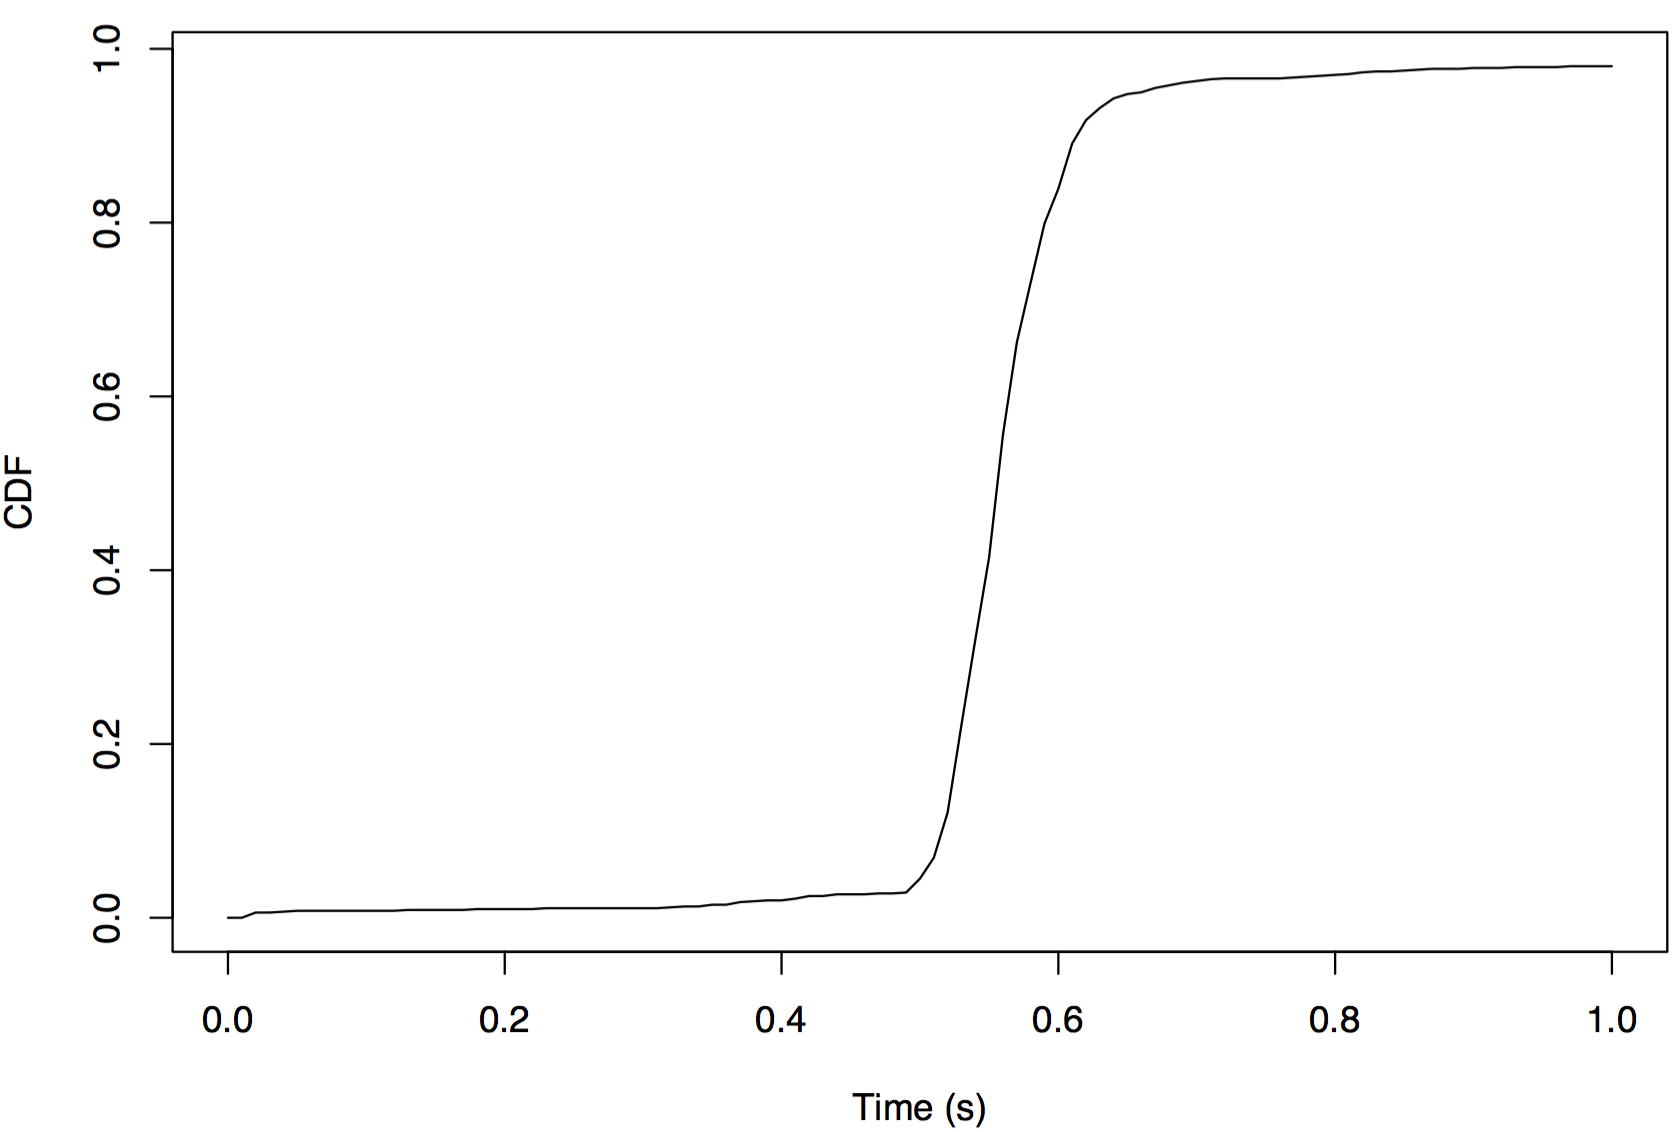
\includegraphics[width=80mm]{figure/runtime}
\caption{Runtime of AS resilience calculation from a given source AS \label{fig_ascal}}
\end{figure}

\textbf{Security Evaluation}\\
Next, we evaluate the security aspect of the relay selection. We first evaluate the relay selection variance in entropy without doing the clustering in step 4. We use the Gini coefficient as the entropy evaluation metric, as it has been used in previous work to measure anonymity selection in Tor ~\cite{akhoondi2012lastor}. We evaluate five values of $\alpha: \{0, 0.25, 0.5, 0.75, 1\}$. Note that when $\alpha = 0$, it is equivalent to bandwidth-based selection. Figure ~\ref{fig_gini} shows the result. The green line to the right is when $\alpha = 0$, so it's solely based on bandwidth resulting in a Gini coefficient of $0.607$ for all source ASes. It is interesting that the Gini coefficients for the other four $\alpha$ values which involve resilience-based selection are very similar, all with much lower Gini coefficients (higher entropy and lower skew in relay selection probability) than bandwidth-based selection. 

\begin{figure}[ht!]
\centering
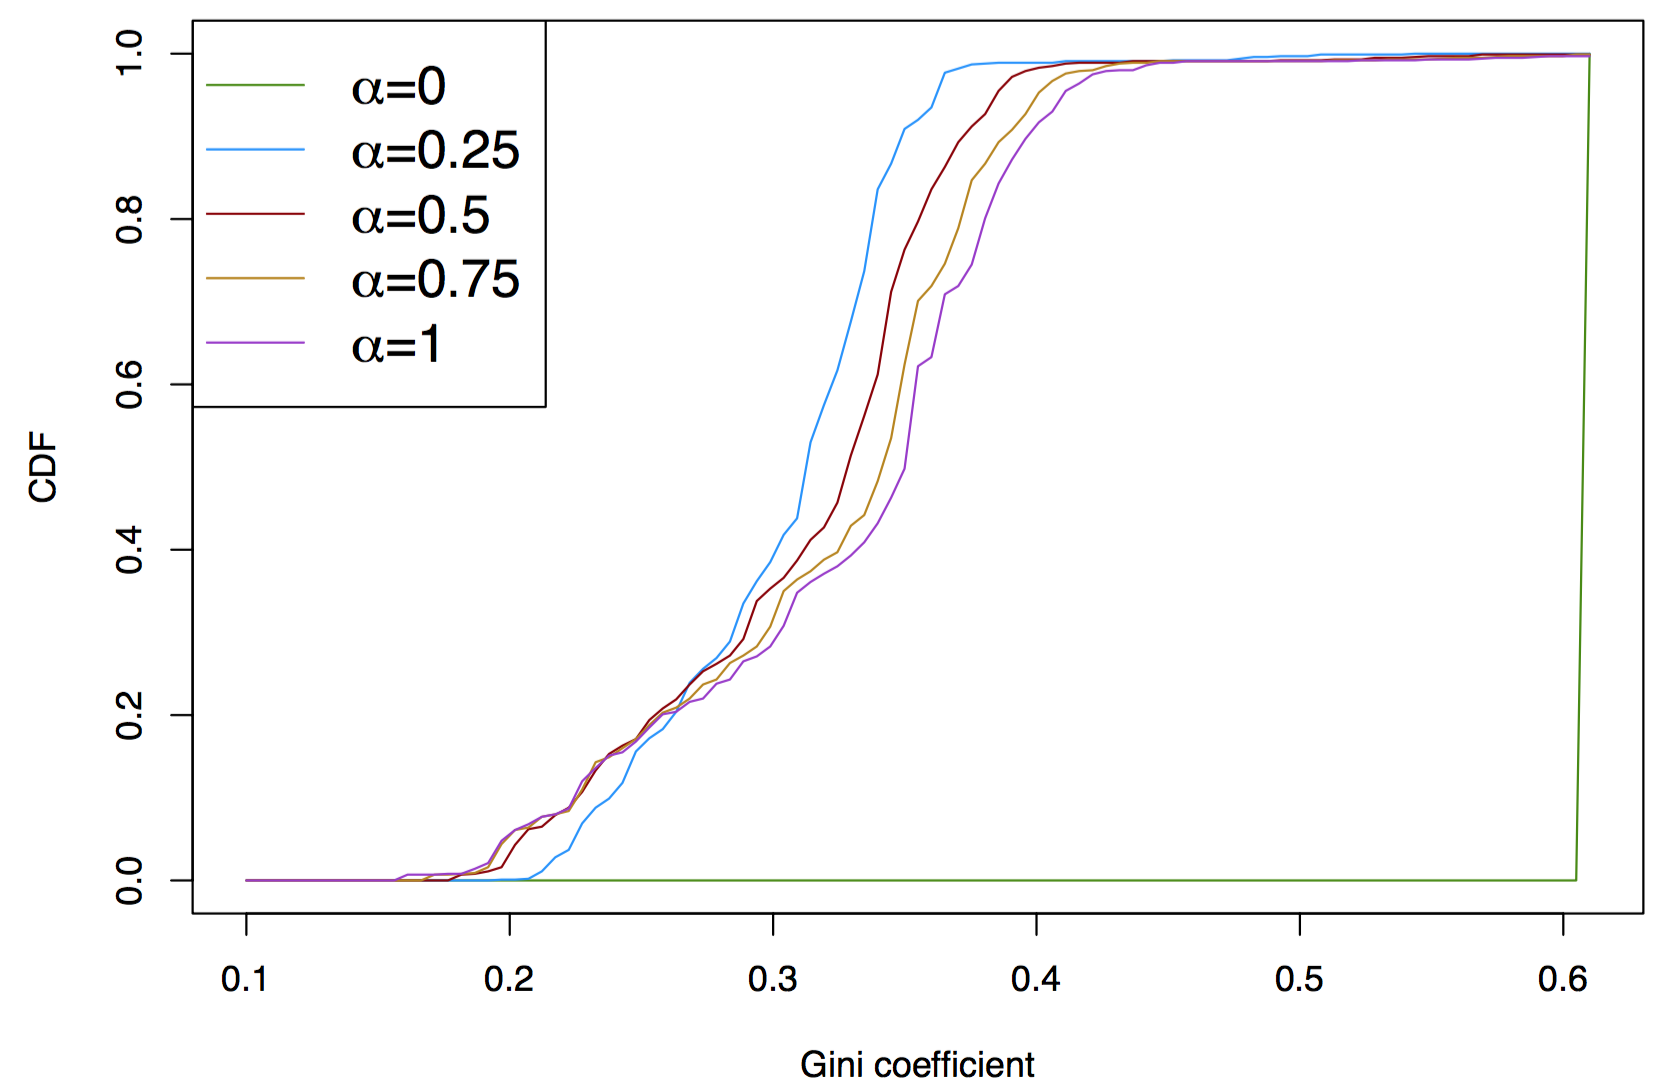
\includegraphics[width=80mm]{figure/gini}
\caption{Gini coefficients with different $\alpha$ values \label{fig_gini}}
\end{figure}




